\documentclass{article}

\usepackage{tikz}
\usetikzlibrary{trees,backgrounds}
\usepackage[paperwidth=25cm,paperheight=22cm,left=1cm,top=1cm]{geometry}

\begin{document}

\sf

\pagestyle{empty}
\tikzstyle{level 1}=[sibling angle=120,level distance=3.5cm]
\tikzstyle{level 2}=[sibling angle=60,level distance=3cm]
\tikzstyle{level 3}=[sibling angle=60]
\tikzstyle{every node}=[fill,text width=2cm,align=center]
\tikzstyle{edge from parent}=[draw,color=black]
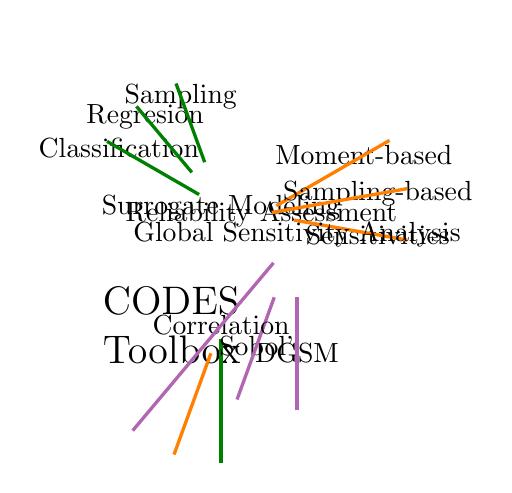
\begin{tikzpicture}[very thick,shape=circle]
	\node[color=blue!50,text=black,text width=3cm,font=\Large ]{CODES Toolbox}
	[clockwise from=90]
	child[color=green!50!black,text=black]{
		node{Surrogate Modeling}
			[clockwise from=150]
			child[color=green!50!black,text=black]{
				node{Classification}
			}
			child[color=green!50!black,text=black]{
				node{Regresion}
			}
			child[color=green!50!black,text=black]{
				node{Sampling}
			}
	}
%	child\texttt{[color=blue!50!green!50!gray,text=black]{
%		node{Multi-Fidelity}
%		[clockwise from=24]
%		child[color=blue!50!green!50!gray,text=black]{
%			node(moment){Contour Estimation}
%		}
%	}
	child[color=orange,text=black]{
		node{Reliability Assessment}
		[clockwise from=30]
		child[color=orange,text=black]{
			node(moment){Moment-based}
		}
		child[color=orange,text=black]{
			node(sampling){Sampling-based}
		}
		child[color=orange,text=black]{
			node(localSensitivities){Sensitivities}
		}
	}
%	child[color=red!70,text=black]{
%		node{RBDO}
%		[clockwise from=-126]
%		child[color=red!70,text=black]{
%			node(sensitivities){Probability Gradients}
%		}
%	}
	child[color=violet!60,text=black]{
		node[color=violet!60,text=black]{Global Sensitivity Analysis}
		[clockwise from=-90]
		child {
			node[color=violet!60,text=black]{DGSM}
		}
		child {
			node[color=violet!60,text=black]{Sobol'}
		}
		child {
			node[color=violet!60,text=black]{Correlation}
		}
	};
%	\begin{pgfonlayer}{background}
%	\draw [draw,color=black,very thick]
%		(moment) edge (sensitivities)
%		(sampling) edge (sensitivities);
%	\end{pgfonlayer}
\end{tikzpicture}

\end{document}